\documentclass[12pt]{article}
\usepackage{url}
\usepackage{graphicx}
\graphicspath{ {/}}


\title{Fairbook: SDSUI}

\author{A. Snow, C. McKenzie, C. Yang, J. Lyons, M. Zhang}


\begin{document}
	\maketitle
	
	\tableofcontents
		\section{ONIDs}
		snowan, mckencod, yangco, lyonsja, zhangm4


	\section{User Interface Prototypes}


		\subsection{Search/Main Page}
		\includegraphics[width=14cm]{main_page.eps}
			\par
			From this page, the user is able to search for books they would like to purchase. 
			They can use the filters located on the left side of the page to refine their search. 
			In the top right hand corner, the user can access their account settings--and just below that, their cart. 
			The green circle in the lower right hand corner will bring up a modal for the user to sell their book. 
			If they click on an individual book displayed in the main viewing area, they will be taken to the detailed book view page.

		\subsection{Book View Page}
		\includegraphics[width=12cm]{book_view_page.eps}
			\par
			This page displays a larger image of the book and also provides some more detailed information about it. 
			To the right, there is a list of people who are selling that book. 
			Clicking on one of the elements in the list will bring up a confirmation dialog asking if the user wants to add that book to their cart.

		\subsection{Account Page}
		\includegraphics[width=14cm]{account_page.eps}


		\subsection{Selling Dialog Modal}
		\includegraphics[width=14cm]{selling_dialog_modal.eps}


		\subsection{Cart Page}
		\includegraphics[width=10cm]{cart_page.eps}
		\par
		From this page, the user is able to view the books they have added to their cart. 
		The user can remove any books that they no longer want by clicking on the [x] next to each one. 
		They can also choose to proceed to checkout or return to the main page.

	\section{Class Diagrams}

	\includegraphics[width=14cm]{class_diagrams.eps}



	\section{Sequence Diagrams}

		\subsection{Use Case \#1: Search/Buy books}
		\includegraphics[width=14cm]{sequence_diagram1.eps}


		\subsection{Use case \#2: Offer books}
		%\includegraphics[width=14cm]{sequence_diagrams2.eps}


		\subsection{Use case \#3: Manage the app}
		\includegraphics[width=14cm]{sequence_diagram3.eps}


	\section{Meeting Report}
		\subsection{Progress Made}
			Not all group members were able to meet in person, but we utilized our group text to keep everyone informed. 
			This meeting we majorly covered how to divide the workload for this project--SDSUI. 
			We decided that more people would work on UI design, since it represents the bulk of the assignment. 
			Similarly to last time, we are keeping with the plan of having all work/documents on google drive so that every member has a chance to review them. 
			We also realized that we wanted to include one more important section of the UI: a page for the user’s cart of books.


		\subsection{Plans/Goals for Next Week}

		As next week\textquotestingle s information has not yet been published on Canvas, we are not sure exactly what is coming up. 
		However, we plan to get an HTML skeleton created based off of our mockups. 
		Also, we would like to finalize which tools/framework we will be utilizing for this project. 
		This is because we would like to maximize productivity and minimize confusion.

		\subsection{Contributions of each team member}
		\par
		UI Prototypes--Jacob, Cody, Cong \par
		Class Diagram--Andrew \par
		Sequence Diagrams--Jacob, Cody \par
		Meeting Report--Jacob \par
		LaTeX--Jacob 



\end {document}